\chapter{Attaque SSLstrip}

\begin{figure}[H]
  \caption{Attaque SSLstrip (diagramme Dia)}
  \fbox{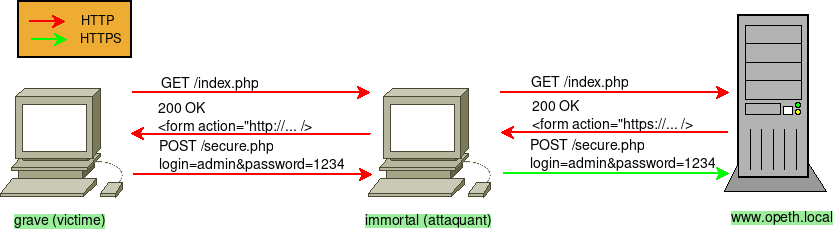
\includegraphics[width=\textwidth]{./sslstrip.png}}
\end{figure}

Le But de l'attaque est de rediriger tout trafic https vers du http sans que la victime s'en aperçoive.

Il faut transformer tous les liens https en http et il faudra garder en mémoire tous les changement effectués.

Pour cela, il faut d'abord mettre en place le Man in the Middle.

Il faut donc mettre en place un ARP poisonning qui va se charger de faire croire à la victime que notre addresse MAC est celle du routeur.

L'attaque doit se passer soit lors des redirections 302, soit quand l'utilisateur clique sur un lien HTTPS.

Les actions à mettre en place :
1. Regarder le trafic HTTP
2. Changer les liens https par des https et garder en mémoire les actions
3. Lorsque qu'on voit une requête HTTP pour une URL que l'on a supprimé, il faut envoyer au serveur du HTTPS
4. Conserver une carte des liens relatifs, CSS, JavaScript
5. Pour essayer de conserver le même aspect visuel, on doit faire de même pour les favicon en renvoyant la favicon de notre choix.
6. A éliminer des en-têtes de requêtes, les encodages, les cookies et les pages en cache.
7. Lors des requêtes POST envoyées par SSL, avec login et password, il faut faire expirer les cookies pour que l'utilisateur renvoie une requête sans cookies
